%\documentclass[hyperref={pdfpagelabels=false},slidetop,9pt]{beamer}
\documentclass[slidetop,8pt]{beamer}
\usepackage[T1]{fontenc}
\usepackage[utf8]{inputenc}
\newcommand{\nom}{Porte conteneur}
\newcommand{\sequence}{03}
\newcommand{\num}{04}
\newcommand{\type}{TD}
\newcommand{\descrip}{Résolution d'un problème en utilisant des méthodes algorithmiques}
\newcommand{\competences}{Alt-C3: Concevoir un algorithme répondant à un problème précisément posé}
\usepackage{etex}
\usepackage{tikz}
\usepackage[european]{circuitikz}
\usepackage{pgf}
\usepackage[all]{xy}
\usepackage{pgfpages}
\usepackage{graphbox}
\usepackage{pdfpages}
\usepackage[adobe-utopia]{mathdesign}
\usepackage{ifthen}
\usepackage{cancel}
\usepackage{framed}
\usepackage{subfig}
\usepackage{tabularx}
\usepackage{setspace}
\usepackage{soul}
\usepackage{schemabloc}
\usepackage{eqnarray}
\usepackage[dot, phantomtext]{dashundergaps}
\usepackage{media9}
\usepackage{multimedia}

\author{Renaud Costadoat}
\institute{Lycée Dorian}

\usepackage{multido}
\usepackage{multirow}
\usepackage{multicol} % Portions de texte en colonnes
\usepackage{flafter}%floatants après la référence

\usepackage{color}
\usepackage{xcolor}
\usepackage{colortbl}

\usepackage[gen]{eurosym}
\usepackage{tikz}
%\usepackage{pstricks,pst-node,pst-tree,pst-solides3d}
\usepackage{lmodern}
\usepackage[francais]{babel}
\usepackage{pslatex}
\usetheme{renaud}
\usepackage{times}
\usepackage{amsmath}
\usepackage{verbatim}
\usepackage{moreverb}
%\usetikzlibrary{arrows,shapes}
\usepackage{graphicx}
\usepackage{psfrag}
\usepackage{wrapfig}
\usepackage{etoolbox}

\definecolor{gris25}{gray}{0.75}
\definecolor{bleu}{RGB}{18,33,98}
\definecolor{bleuf}{RGB}{42,94,171}
\definecolor{bleuc}{RGB}{231,239,247}
\definecolor{rougef}{RGB}{185,18,27}
\definecolor{rougec}{RGB}{255,188,204}%255,230,231
\definecolor{vertf}{RGB}{103,126,82}
\definecolor{vertc}{RGB}{220,255,191}

\setlength\parindent{24pt}
\parskip 7.2pt
\parindent 8pt

\newenvironment{rem}[1][\hsize]%
{%
    \def\FrameCommand
   {%
\rotatebox{90}{\textit{\textsf{Remarque}}} 
       {\color{bleuf}\vrule width 3pt}%
       \hspace{0pt}%must no space.
       \fboxsep=\FrameSep\colorbox{bleuc}%
  }%
    \MakeFramed{\hsize#1\advance\hsize-\width\FrameRestore}%
}%
{\endMakeFramed}%


\newenvironment{savoir}[1][\hsize]%
{%
    \def\FrameCommand
    {%
\rotatebox{90}{\textit{\textsf{Savoir}}} 
        {\color{bleuf}\vrule width 3pt}%
        \hspace{0pt}%must no space.
        \fboxsep=\FrameSep\colorbox{bleuc}%
    }%
    \MakeFramed{\hsize#1\advance\hsize-\width\FrameRestore}%
}%
{\endMakeFramed}%

\newenvironment{prob}[1][\hsize]%
{%
    \def\FrameCommand%
    {%
\rotatebox{90}{\textit{\textsf{Problématique}}} 
        {\color{rougef}\vrule width 3pt}%
        \hspace{0pt}%must no space.
        \fboxsep=\FrameSep\colorbox{rougec}%
    }%
    \MakeFramed{\hsize#1\advance\hsize-\width\FrameRestore}%
}%
{\endMakeFramed}%

\newenvironment{obj}[1][\hsize]%
{%
    \def\FrameCommand%
    {%
\rotatebox{90}{\textit{\textsf{Objectif}}} 
        {\color{vertf}\vrule width 3pt}%
        \hspace{0pt}%must no space.
        \fboxsep=\FrameSep\colorbox{vertc}%
    }%
    \MakeFramed{\hsize#1\advance\hsize-\width\FrameRestore}%
}%
{\endMakeFramed}%

\newenvironment{defi}[1][\hsize]%
{%
    \def\FrameCommand%
    {%
\rotatebox{90}{\textit{\textsf{Definition}}} 
        {\color{bleuf}\vrule width 3pt}%
        \hspace{0pt}%must no space.
        \fboxsep=\FrameSep\colorbox{rougec}%
    }%
    \MakeFramed{\hsize#1\advance\hsize-\width\FrameRestore}%
}%
{\endMakeFramed}%


\newenvironment{hypo}[1][\hsize]%
{%
    \def\FrameCommand%
    {%
\rotatebox{90}{\textit{\textsf{Hypothèse\\}}} 
        {\color{bleuf}\vrule width 3pt}%
        \hspace{0pt}%must no space.
        \fboxsep=\FrameSep\colorbox{bleuc}%
    }%
    \MakeFramed{\hsize#1\advance\hsize-\width\FrameRestore}%
}%
{\endMakeFramed}%


\newenvironment{prop}[1][\hsize]%
{%
    \def\FrameCommand%
    {%
\rotatebox{90}{\textit{\textsf{Propriété}}} 
        {\color{bleuf}\vrule width 3pt}%
        \hspace{0pt}%must no space.
        \fboxsep=\FrameSep\colorbox{bleuc}%
    }%
    \MakeFramed{\hsize#1\advance\hsize-\width\FrameRestore}%
}%
{\endMakeFramed}%

\newenvironment{props}[1][\hsize]%
{%
    \def\FrameCommand%
    {%
\rotatebox{90}{\textit{\textsf{Propriétés}}} 
        {\color{bleuf}\vrule width 3pt}%
        \hspace{0pt}%must no space.
        \fboxsep=\FrameSep\colorbox{bleuc}%
    }%
    \MakeFramed{\hsize#1\advance\hsize-\width\FrameRestore}%
}%
{\endMakeFramed}%

\newenvironment{exemple}[1][\hsize]%
{%
    \def\FrameCommand%
    {%
\rotatebox{90}{\textit{\textsf{Exemple}}} 
        {\color{vertf}\vrule width 3pt}%
        \hspace{0pt}%must no space.
        \fboxsep=\FrameSep\colorbox{vertc}%
    }%
    \MakeFramed{\hsize#1\advance\hsize-\width\FrameRestore}%
}%
{\endMakeFramed}%

\newenvironment{resultat}[1][\hsize]%
{%
    \def\FrameCommand%
    {%
\rotatebox{90}{\textit{\textsf{Resultat}}} 
        {\color{rougef}\vrule width 3pt}%
%        {\color{bleuf}\vrule width 3pt}%
        \hspace{0pt}%must no space.
        \fboxsep=\FrameSep\colorbox{rougec}%
    }%
    \MakeFramed{\hsize#1\advance\hsize-\width\FrameRestore}%
}%
{\endMakeFramed}%

\newenvironment{methode}[1][\hsize]%
{%
    \def\FrameCommand%
    {%
\rotatebox{90}{\textit{\textsf{Méthode\\}}} 
        {\color{rougef}\vrule width 3pt}%
        \hspace{0pt}%must no space.
        \fboxsep=\FrameSep\colorbox{rougec}%
    }%
    \MakeFramed{\hsize#1\advance\hsize-\width\FrameRestore}%
}%
{\endMakeFramed}%

\newenvironment{theo}[1][\hsize]%
{%
    \def\FrameCommand%
    {%
\rotatebox{90}{\textit{\textsf{Théorème\\}}} 
        {\color{rougef}\vrule width 3pt}%
        \hspace{0pt}%must no space.
        \fboxsep=\FrameSep\colorbox{rougec}%
    }%
    \MakeFramed{\hsize#1\advance\hsize-\width\FrameRestore}%
}%
{\endMakeFramed}%

\newenvironment{warn}[1][\hsize]%
{%
    \def\FrameCommand%
    {%
\rotatebox{90}{\textit{\textsf{Attention\\}}} 
        {\color{rougef}\vrule width 3pt}%
        \hspace{0pt}%must no space.
        \fboxsep=\FrameSep\colorbox{rougec}%
    }%
    \MakeFramed{\hsize#1\advance\hsize-\width\FrameRestore}%
}%
{\endMakeFramed}%

% \usepackage{pstricks}
%\usepackage{minitoc}
% \setcounter{minitocdepth}{4}

\setcounter{tocdepth}{2}

% \mtcselectlanguage{french} 

%\usepackage{draftcopy}% "Brouillon"
% \usepackage{floatflt}
\usepackage{psfrag}
%\usepackage{listings} % Permet d'insérer du code de programmation
\renewcommand{\baselinestretch}{1.2}

% Changer la numérotation des figures :
% ------------------------------------
% \makeatletter
% \renewcommand{\thefigure}{\ifnum \c@section>\z@ \thesection.\fi
%  \@arabic\c@figure}
% \@addtoreset{figure}{section}
% \makeatother
 


%%%%%%%%%%%%
% Définition des vecteurs %
%%%%%%%%%%%%
 \newcommand{\vect}[1]{\overrightarrow{#1}}

%%%%%%%%%%%%
% Définition des torseusr %
%%%%%%%%%%%%

 \newcommand{\torseur}[1]{%
\left\{{#1}\right\}
}

\newcommand{\torseurcin}[3]{%
\left\{\mathcal{#1} \left(#2/#3 \right) \right\}
}

\newcommand{\torseurstat}[3]{%
\left\{\mathcal{#1} \left(#2\rightarrow #3 \right) \right\}
}

 \newcommand{\torseurc}[8]{%
%\left\{#1 \right\}=
\left\{
{#1}
\right\}
 = 
\left\{%
\begin{array}{cc}%
{#2} & {#5}\\%
{#3} & {#6}\\%
{#4} & {#7}\\%
\end{array}%
\right\}_{#8}%
}

 \newcommand{\torseurcol}[7]{
\left\{%
\begin{array}{cc}%
{#1} & {#4}\\%
{#2} & {#5}\\%
{#3} & {#6}\\%
\end{array}%
\right\}_{#7}%
}

 \newcommand{\torseurl}[3]{%
%\left\{\mathcal{#1}\right\}_{#2}=%
\left\{%
\begin{array}{l}%
{#1} \\%
{#2} %
\end{array}%
\right\}_{#3}%
}

 \newcommand{\vectv}[3]{%
\vect{V\left( {#1} \in {#2}/{#3}\right)}
}


\newcommand{\vectf}[2]{%
\vect{R\left( {#1} \rightarrow {#2}\right)}
}

\newcommand{\vectm}[3]{%
\vect{\mathcal{M}\left( {#1}, {#2} \rightarrow {#3}\right)}
}


 \newcommand{\vectg}[3]{%
\vect{\Gamma \left( {#1} \in {#2}/{#3}\right)}
}

 \newcommand{\vecto}[2]{%
\vect{\Omega\left( {#1}/{#2}\right)}
}

\newcommand{\reponse}[1][4]
{
\multido{}{#1}
{
\begin{center}
\makebox[0.9\linewidth]{\dotfill} \end{center}
}}


% }$$\left\{\mathcal{#1} \right\}_{#2} =%
% \left\{%
% \begin{array}{c}%
%  #3 \\%
%  #4 %
% \end{array}%
% \right\}_{#5}}


%  ------------------------------------------
% | Modification du formatage des sections : | 
%  ------------------------------------------

% Grands titres :
% ---------------

\newcommand{\titre}[1]{%
\begin{center}
      \bigskip
      \rule{\textwidth}{1pt}
      \par\vspace{0.1cm}
      
      \textbf{\large #1}
      \par\rule{\textwidth}{1pt}
    \end{center}
    \bigskip
  }

% Supprime le numéro du chapitre dans la numérotation des sections:
% -----------------------------------------------------------------
\makeatletter
\renewcommand{\thesection}{\@arabic\c@section}
\makeatother


% \titleformat{\chapter}[display]
% {\normalfont\Large\filcenter}
% {}
% {1pc}
% {\titlerule[1pt]
%   \vspace{1pc}%
%   \Huge}[\vspace{1ex}%
% \titlerule]


%%%% Chapitres Comme PY Pechard %%%%%%%%%
% numéro du chapitre
\DeclareFixedFont{\chapnumfont}{OT1}{phv}{b}{n}{80pt}
% pour le mot « Chapitre »
\DeclareFixedFont{\chapchapfont}{OT1}{phv}{m}{it}{40pt}
% pour le titre
\DeclareFixedFont{\chaptitfont}{T1}{phv}{b}{n}{25pt}

\definecolor{gris}{gray}{0.75}
\setbeamertemplate{section in toc}[sections numbered]

\newlength{\RoundedBoxWidth}
\newsavebox{\GrayRoundedBox}
\newenvironment{GrayBox}[1][\dimexpr\textwidth-4.5ex]%
   {\setlength{\RoundedBoxWidth}{\dimexpr#1}
    \begin{lrbox}{\GrayRoundedBox}
       \begin{minipage}{\RoundedBoxWidth}}%
   {   \end{minipage}
    \end{lrbox}
    \begin{center}
    \begin{tikzpicture}%
       \draw node[draw=bleuf,fill=bleuc,rounded corners,%
             inner sep=2ex,text width=\RoundedBoxWidth]%
             {\usebox{\GrayRoundedBox}};
    \end{tikzpicture}
    \end{center}}
    
\ifdef{\prive}{\pgfpagesuselayout{2 on 1}[a4paper,border shrink=0mm]}
\ifdef{\prive}{\setbeamertemplate{navigation symbols}{}}
\setbeamertemplate{itemize item}[ball]
%\setbeamertemplate{blocks}[rounded]%[shadow=true]
\setbeamercolor{block title}{fg=white,bg=grisf}        % titre block normal 
\setbeamercolor{block body}{fg=grisf,bg=grisc!50}      % corps block normal
\setbeamercolor{block body alerted}{fg=white,bg=warning}   % idem pour un block alerte

\title{\nom}
\date{S\sequence \ - \type\num}

\begin{document}
\shorthandoff{:!}
\bibliographystyle{abbrvnat-fr}

\usebackgroundtemplate%
{%
    \centering
\includegraphics[width=\paperwidth]{../../img/fond2}%
}

{
\setbeamertemplate{navigation symbols}{}
\setbeamertemplate{headline}[pagetitre]
\setbeamertemplate{footline}[pagetitre]
\usebackgroundtemplate{\centering
\includegraphics[width=\paperwidth]{../../img/fond}}
\frame{\titlepage}
}



\section{Introduction à l'informatique} 

{\frame{
\frametitle{Présentation de l'informatique}

\begin{wrapfigure}[10]{r}{3.5cm}
\vspace{-10mm}
\centering 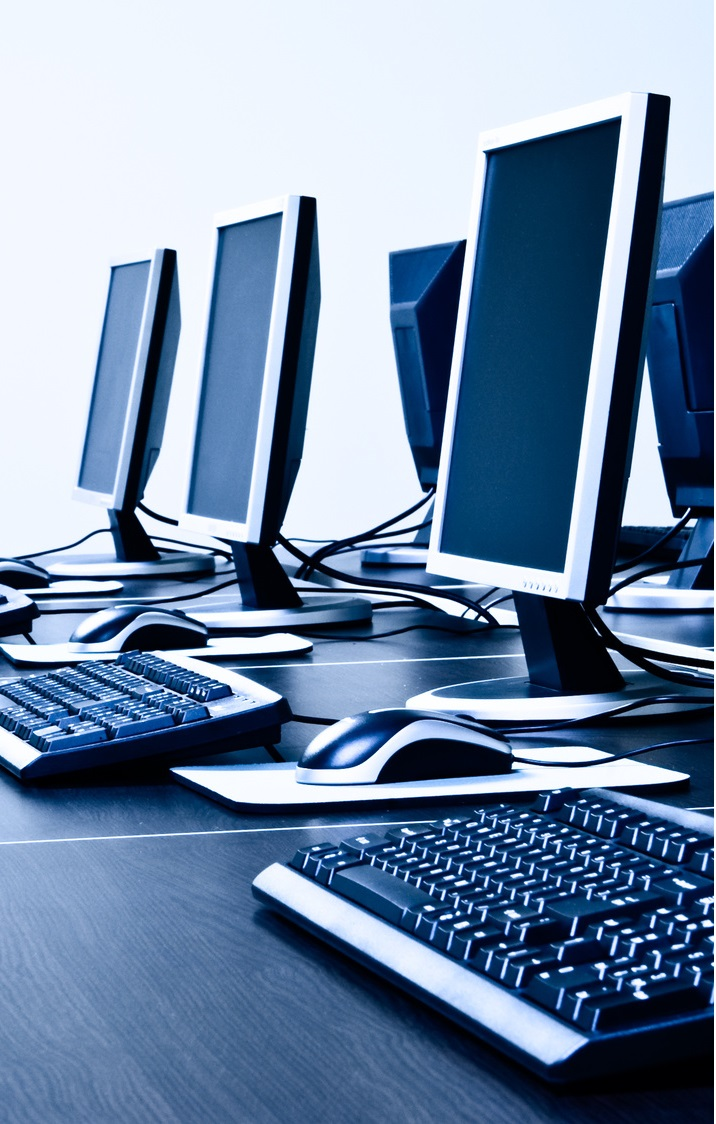
\includegraphics[width=\linewidth]{img/info}
\end{wrapfigure}

L'informatique, omniprésente dans les différentes sphères de l'entreprise, de la recherche,
des services, de la culture et des loisirs, repose sur des mécanismes fondamentaux devant
être maîtrisés par les futurs ingénieurs, enseignants et chercheurs qui auront à s'en servir
pour agir en connaissance de cause dans leur vie professionnelle.

La rapide évolution des outils informatiques et des sciences du numérique dans tous les
secteurs de l'ingénierie (industrielle, logicielle et des services) et de la recherche rend
indispensable un enseignement de l'informatique spécifiquement conçu pour l'étudiant de
CPGE scientifiques.

Au niveau fondamental, on se fixe pour objectif la maîtrise d'un certain nombre de concepts
de base, et avant tout, la conception rigoureuse d'algorithmes et le choix de représentations
appropriées des données. Ceci impose une expérience pratique de la programmation et de
la manipulation informatique de données, notamment d'origine expérimentale ou industrielle,
et parfois disponibles en ligne.

}}


{\frame{
\frametitle{Compétences visées}

Cet enseignement doit permettre de développer les compétences suivantes :
~\

\begin{tabular}{|l|m{7cm}|}
\hline
Analyser et modéliser & un problème, une situation \\
\hline
Imaginer et concevoir & une solution algorithmique modulaire, utilisant des méthodes de programmation, des structures de données appropriées pour le problème étudié \\
\hline
Traduire & un algorithme dans un langage de programmation moderne et généraliste \\
\hline
Spécifier & rigoureusement les modules ou fonctions \\
\hline
Évaluer, contrôler, valider & des algorithmes et des programmes \\
\hline
Communiquer & à l'écrit ou à l'oral, une problématique, une solution ou un algorithme, une documentation \\
\hline
\end{tabular}




}}

\section{Traitement de l'information} 
 
 
{\frame{
\frametitle{Technologie informatique}

Elles sont basées sur l'interaction entre :
\begin{itemize}
 \item Des \textbf{programmes}, aussi appelés logiciels ou applications, décrivant des processus de traitement de l'information : biens immatériels,
 \item Des \textbf{ordinateurs}, capables d'exécuter ces programmes : biens matériels.
\end{itemize}

~\

\begin{minipage}{0.24\linewidth}
 
\includegraphics[width=0.7\linewidth]{img/gimp}
\end{minipage}\hfill
\begin{minipage}{0.24\linewidth}
 
\includegraphics[width=0.7\linewidth]{img/linux}
\end{minipage}\hfill
\begin{minipage}{0.24\linewidth}
 
\includegraphics[width=0.7\linewidth]{img/windows10}
\end{minipage}\hfill
\begin{minipage}{0.24\linewidth}
 
\includegraphics[width=0.7\linewidth]{img/batman}
\end{minipage}

\begin{minipage}{0.24\linewidth}
 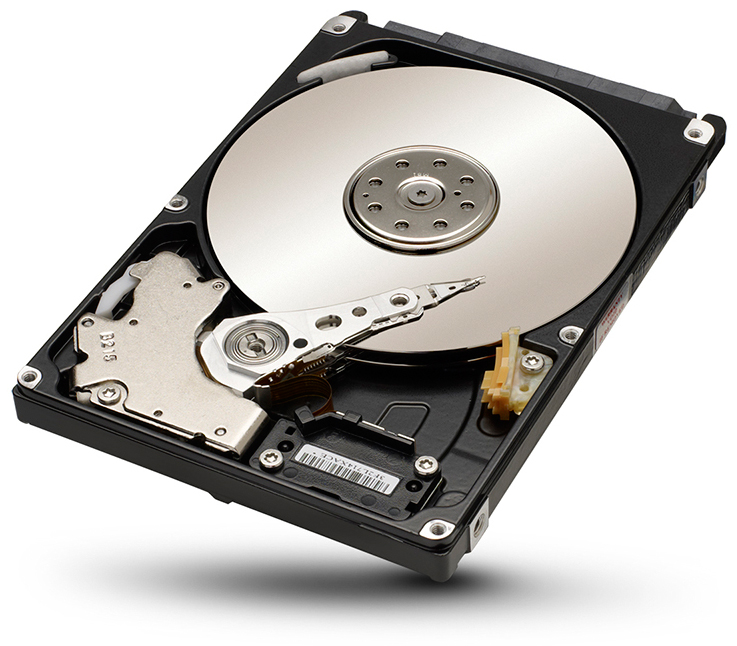
\includegraphics[width=0.7\linewidth]{img/disque_dur}
\end{minipage}\hfill
\begin{minipage}{0.24\linewidth}
 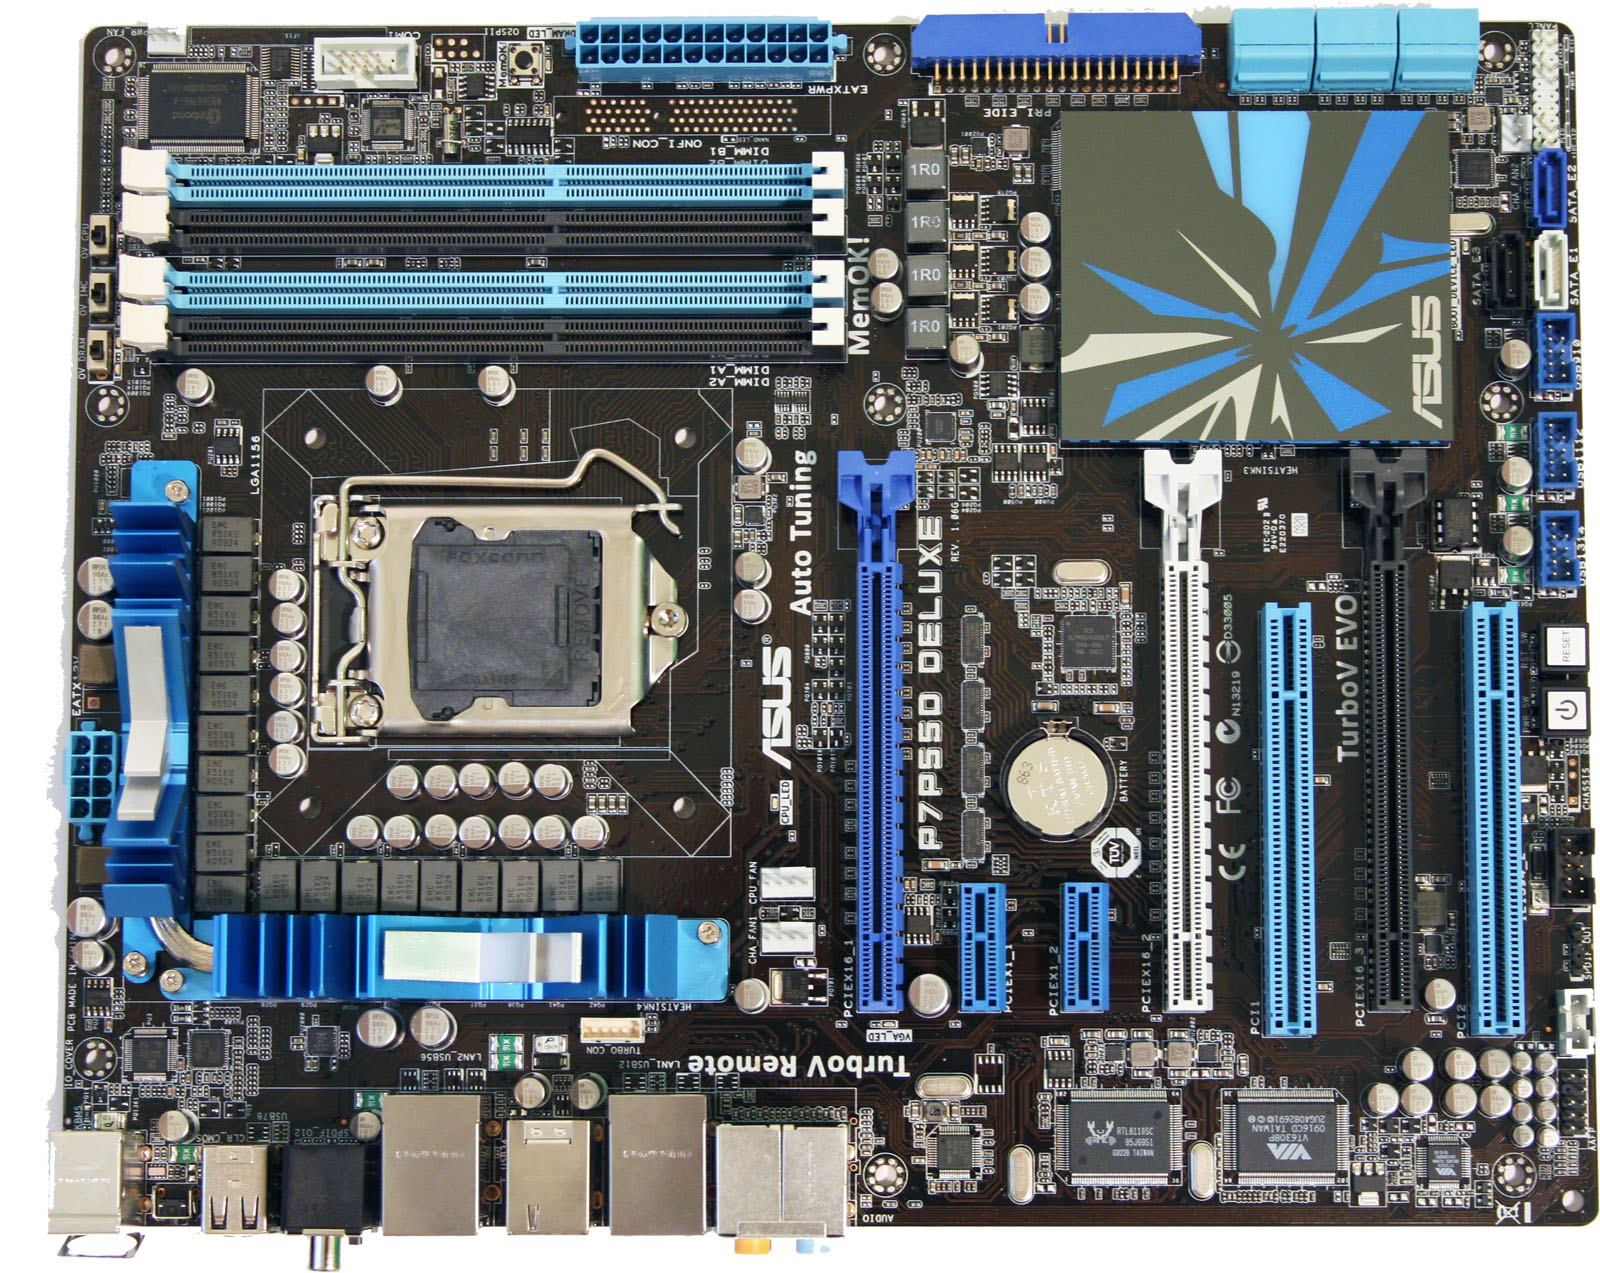
\includegraphics[width=0.7\linewidth]{img/carte_mere}
\end{minipage}\hfill
\begin{minipage}{0.24\linewidth}
 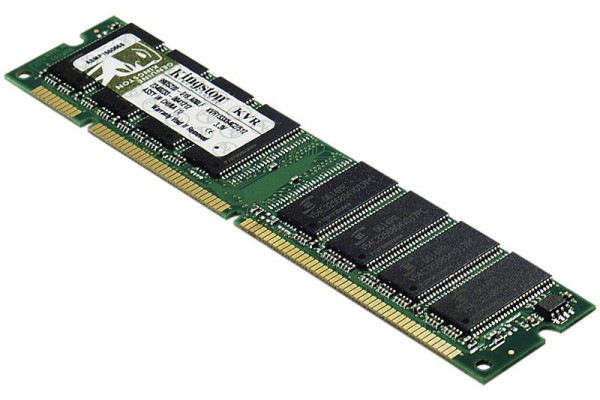
\includegraphics[width=0.7\linewidth]{img/ram}
\end{minipage}\hfill
\begin{minipage}{0.24\linewidth}
 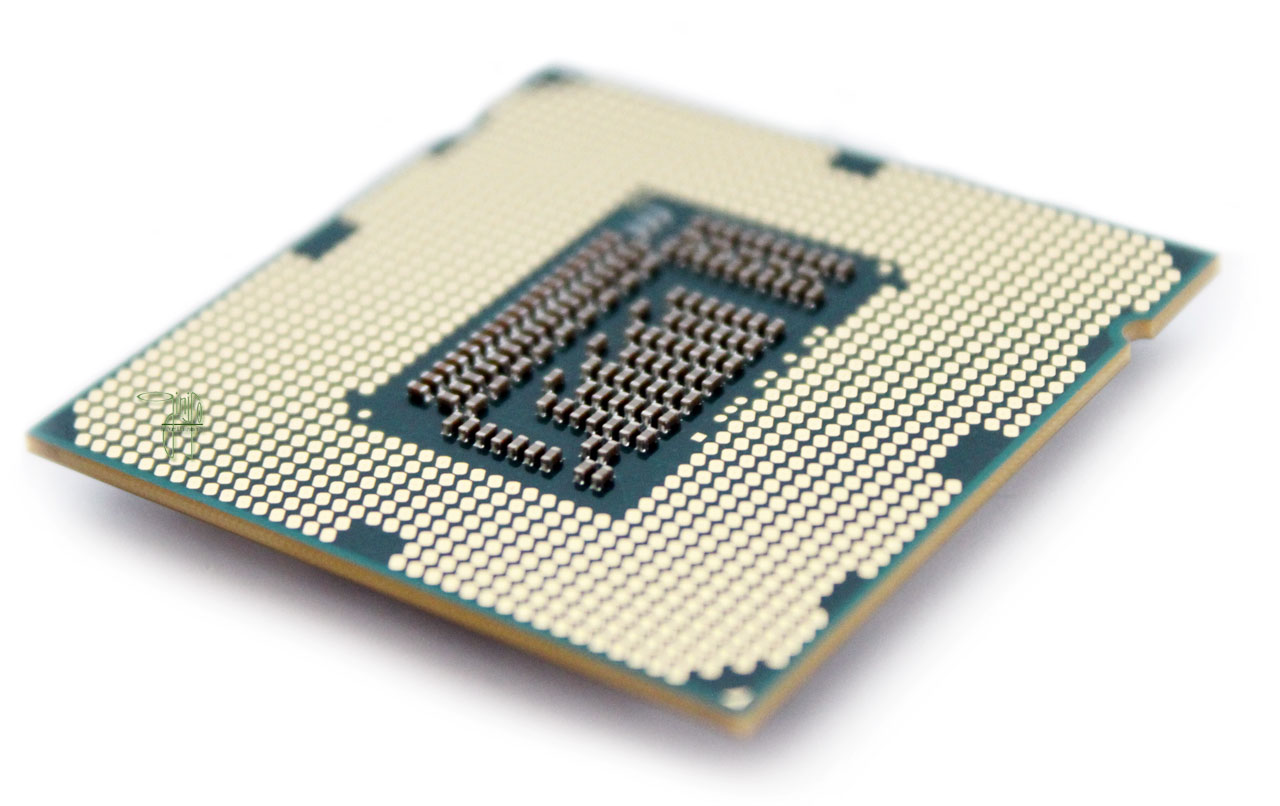
\includegraphics[width=0.7\linewidth]{img/processeur}
\end{minipage}

}}

{\frame{
\frametitle{Parcours de l'information}

Un ordinateur est une machine programmable de traitement de l'information.

~\

La chaîne de traitement de l'information est composée des fonctions suivantes:
\begin{itemize}
 \item \textbf{Acquérir} de l'information de l'extérieur,
 \item \textbf{Stocker} en son sein ces informations,
 \item \textbf{Traiter} les informations à sa disposition,
 \item \textbf{Restituer} ces informations à l'extérieur.
\end{itemize}

~\

\begin{center}
 \begin{tikzpicture}
 \node[draw, bleuf] (P) at (0,0) {Acquérir};
 \node[draw, bleuf] (S) at (2,0) {Stocker};
 \node[draw, bleuf] (T) at (4,0) {Traiter};
 \node[draw, bleuf] (R) at (6,0) {Restituer};
 \draw[->,>=latex, bleuf] (P) |- (S);
 \draw[->,>=latex, bleuf] (S) |- (T);
 \draw[->,>=latex, bleuf] (T) |- (R);
 \end{tikzpicture}
\end{center}
}}

{\frame{
\frametitle{Instruction}

Une instruction est l'opération élémentaire que le processeur peut accomplir. Les instructions sont stockées dans la mémoire principale, en vue d'être traitée par le processeur. Une instruction est composée de deux champs :
\begin{itemize}
 \item le code \textbf{opération}, représentant l'action que le processeur doit accomplir ;
 \item le code \textbf{opérande}, définissant les paramètres de l'action. Le code opérande dépend de l'opération. Il peut s'agir d'une donnée ou bien d'une adresse mémoire.
\end{itemize}

~\

Les instructions peuvent être classées en catégories dont les principales sont :
\begin{itemize}
 \item \textbf{Accès à la mémoire} : des accès à la mémoire ou transferts de données entre registres.
 \item \textbf{Opérations arithmétiques} : opérations telles que les additions, soustractions, divisions ou multiplication.
 \item \textbf{Opérations logiques} : opérations ET, OU, NON, NON exclusif, etc.
 \item \textbf{Contrôle} : contrôles de séquence, branchements conditionnels, etc.
\end{itemize}
}}

{\frame{
\frametitle{Systèmes multi-couches}

\begin{wrapfigure}[13]{r}{3cm}
\vspace{-7mm}
 \begin{tikzpicture}
 \node[draw, bleuf] (1) at (0,5) {Langage d'application};
 \node[draw, bleuf] (2) at (0,4) {Langage d'assemblage};
 \node[draw, bleuf] (3) at (0,3) {Système d'exploitation};
 \node[draw, bleuf] (4) at (0,2) {Jeu d'instruction};
 \node[draw, bleuf] (5) at (0,1) {Micro architecture};
 \node[draw, bleuf] (6) at (0,0) {Logique numérique};
 \draw[->,>=latex, bleuf] (1) -- (2);
 \draw[->,>=latex, bleuf] (2) -- (3);
 \draw[->,>=latex, bleuf] (3) -- (4);
 \draw[->,>=latex, bleuf] (4) -- (5);
 \draw[->,>=latex, bleuf] (5) -- (6);
 \end{tikzpicture}
\end{wrapfigure}


Les processeurs ne comprennent que le langage machine.

Exemple d'instruction pour un microprosseur de la famille x86 (32bits): \texttt{10110000 01100001}

~\

Ce langage est trop élémentaire, trop long à programmer, il est donc nécessaire de construire des programmes à un niveau d'abstraction plus élevé, afin d'avoir:
\begin{itemize}
 \item Meilleure expressivité et généricité,
 \item Moins de risques d'erreurs,
 \item Besoin de passer d'un langage humainement compréhensible à une exécution machine.
\end{itemize}

\begin{center}
Cela a favorisé la conception de systèmes, \textbf{multi-couches}.
\end{center}
}}

{\frame{
\frametitle{Systèmes multi-couches}

\textbf{Couche logique numérique:} Portes logiques (construites à partir de transistors) qui calculent en sortie une fonction logique simple (ET, OU, NON).

\textbf{Couche microarchitecture:} Ce niveau contient plusieurs registres mémoire et un circuit (appelé UAL) capable de réaliser des opérations arithmétiques élémentaires

\textbf{Couche jeu d'instruction:} La couche de l'architecture du jeu d'instructions est définie par le jeu des instructions disponibles sur la machine.

\textbf{Couche système d'exploitation:} Cette couche permet de bénéficier des services offerts par le système d'exploitation.

\textbf{Couche langage d'assemblage:} Offre une forme symbolique aux langages des couches inférieures et permet à des humains d'interagir avec les couches inférieures.

\textbf{Couche langages d'application:} Met à la disposition des programmeurs d'applications un ensemble de langages adaptés à leurs besoins.
Ce sont les langages dits \og de haut niveau \fg.
}}

\section{Architecture des ordinateurs} 

{\frame{
\frametitle{Systèmes informatiques}
Les systèmes informatiques prennent plusieurs formes et sont très présents dans notre quotidien.

~\

\begin{minipage}{0.32\linewidth}
 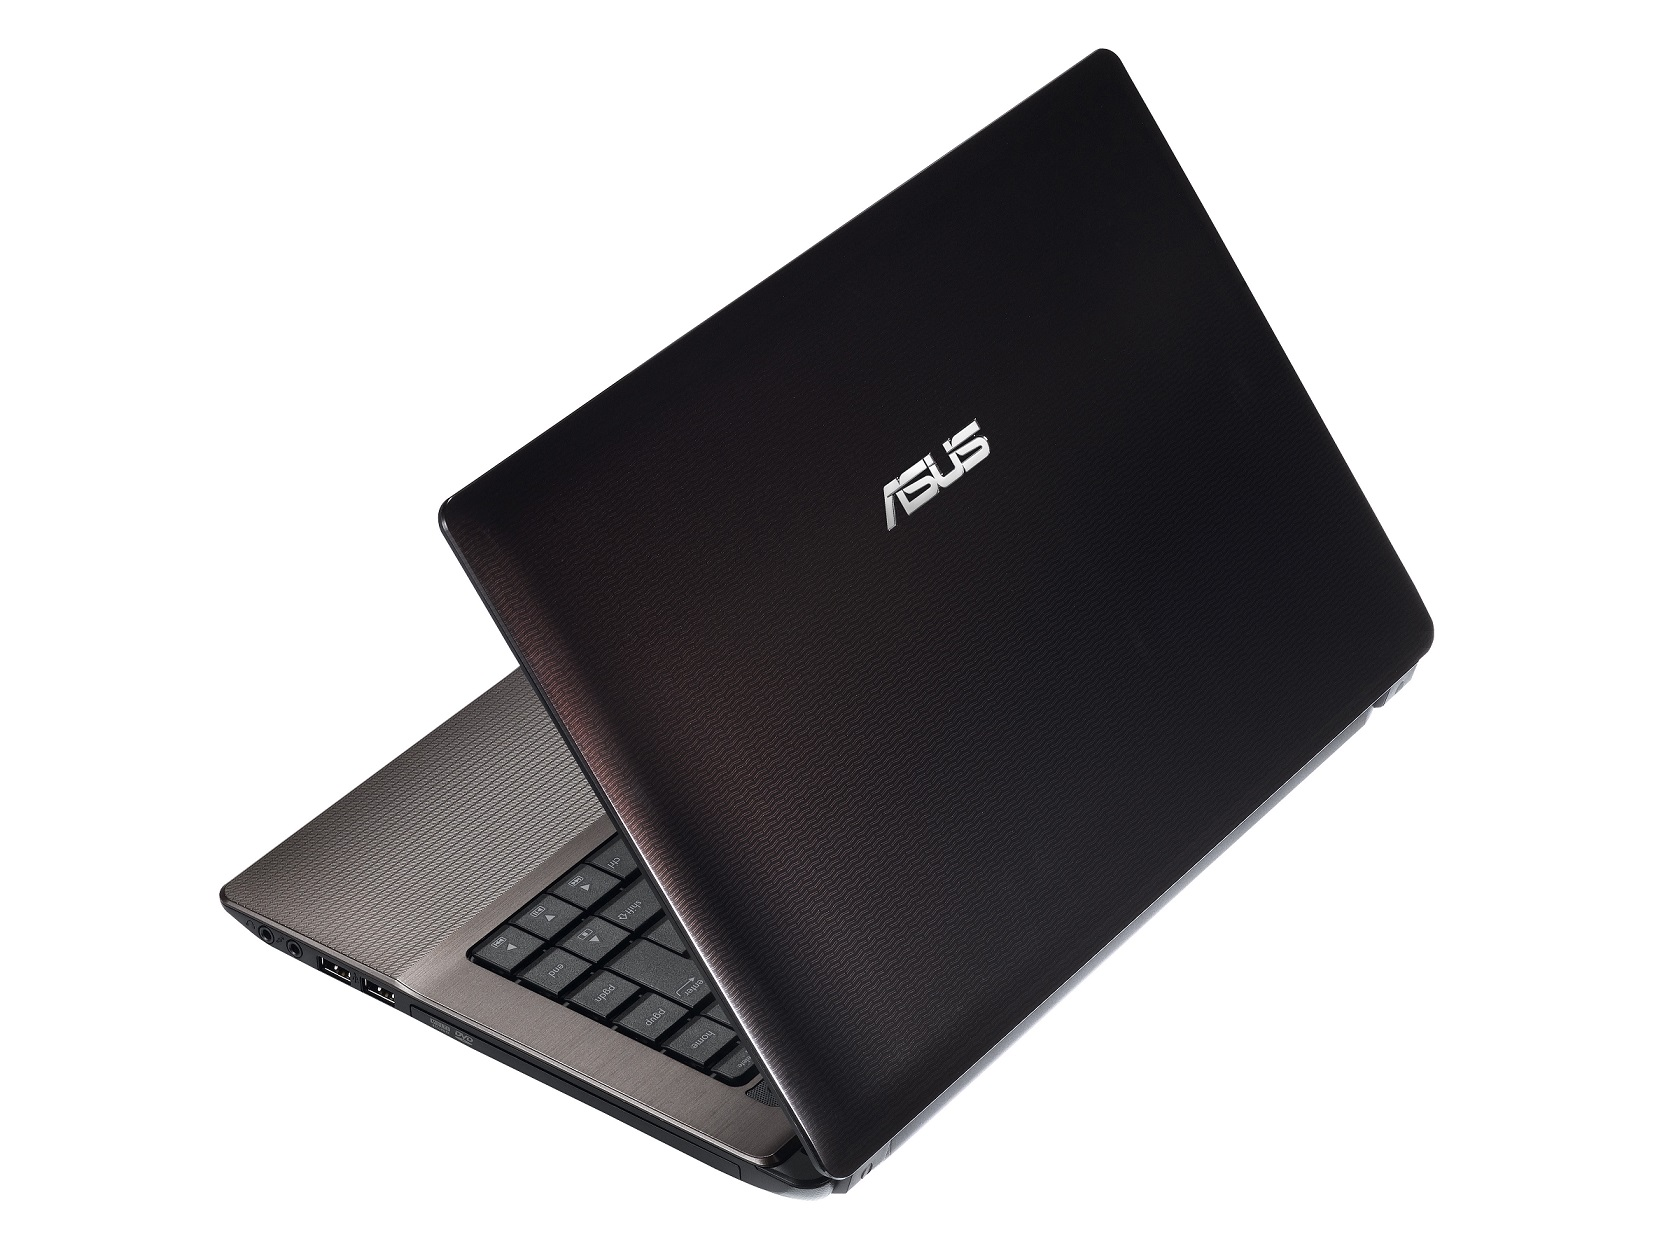
\includegraphics[width=0.7\linewidth]{img/asus}
\end{minipage}\hfill
\begin{minipage}{0.32\linewidth}
 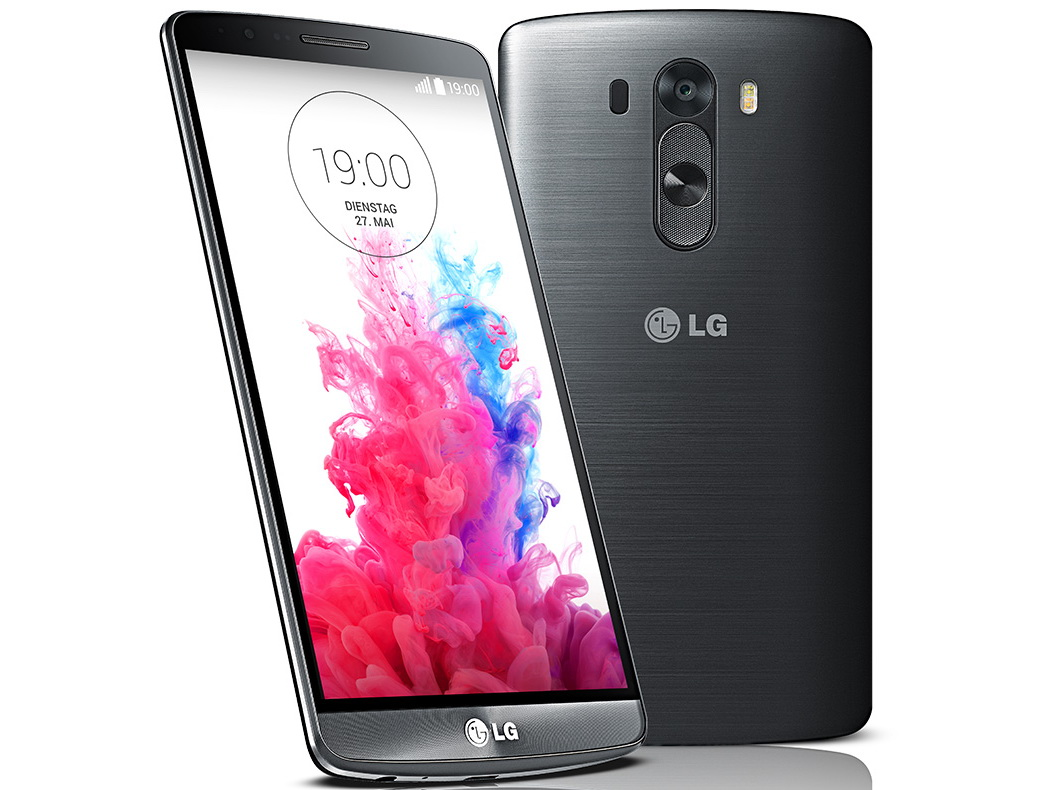
\includegraphics[width=0.7\linewidth]{img/lg-g3}
\end{minipage}\hfill
\begin{minipage}{0.32\linewidth}
 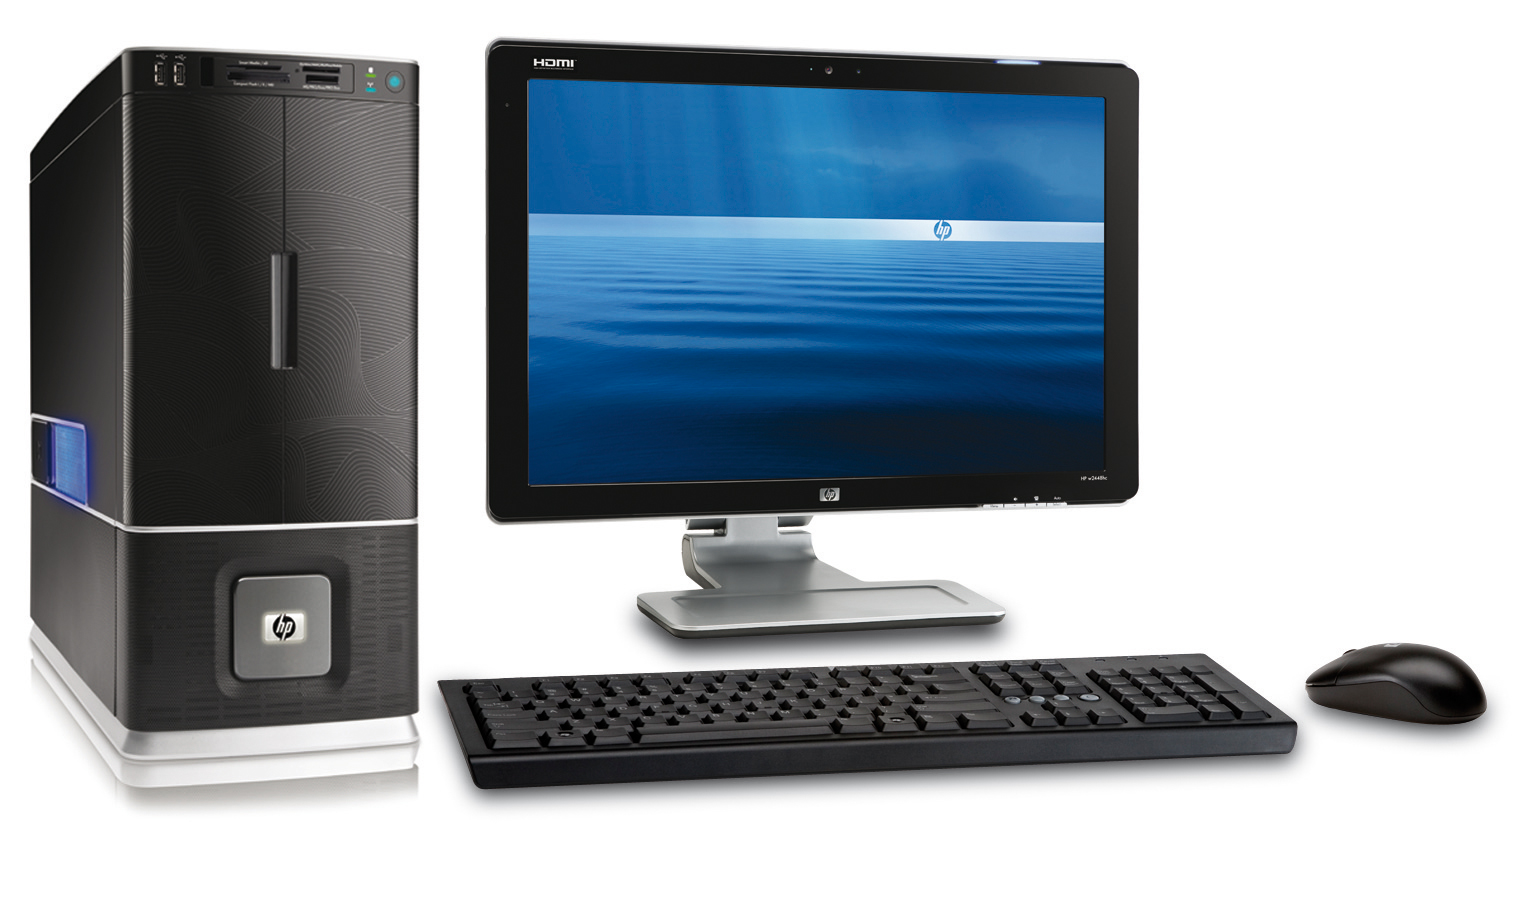
\includegraphics[width=0.7\linewidth]{img/DesktopPC}
\end{minipage}

\begin{minipage}{0.32\linewidth}
 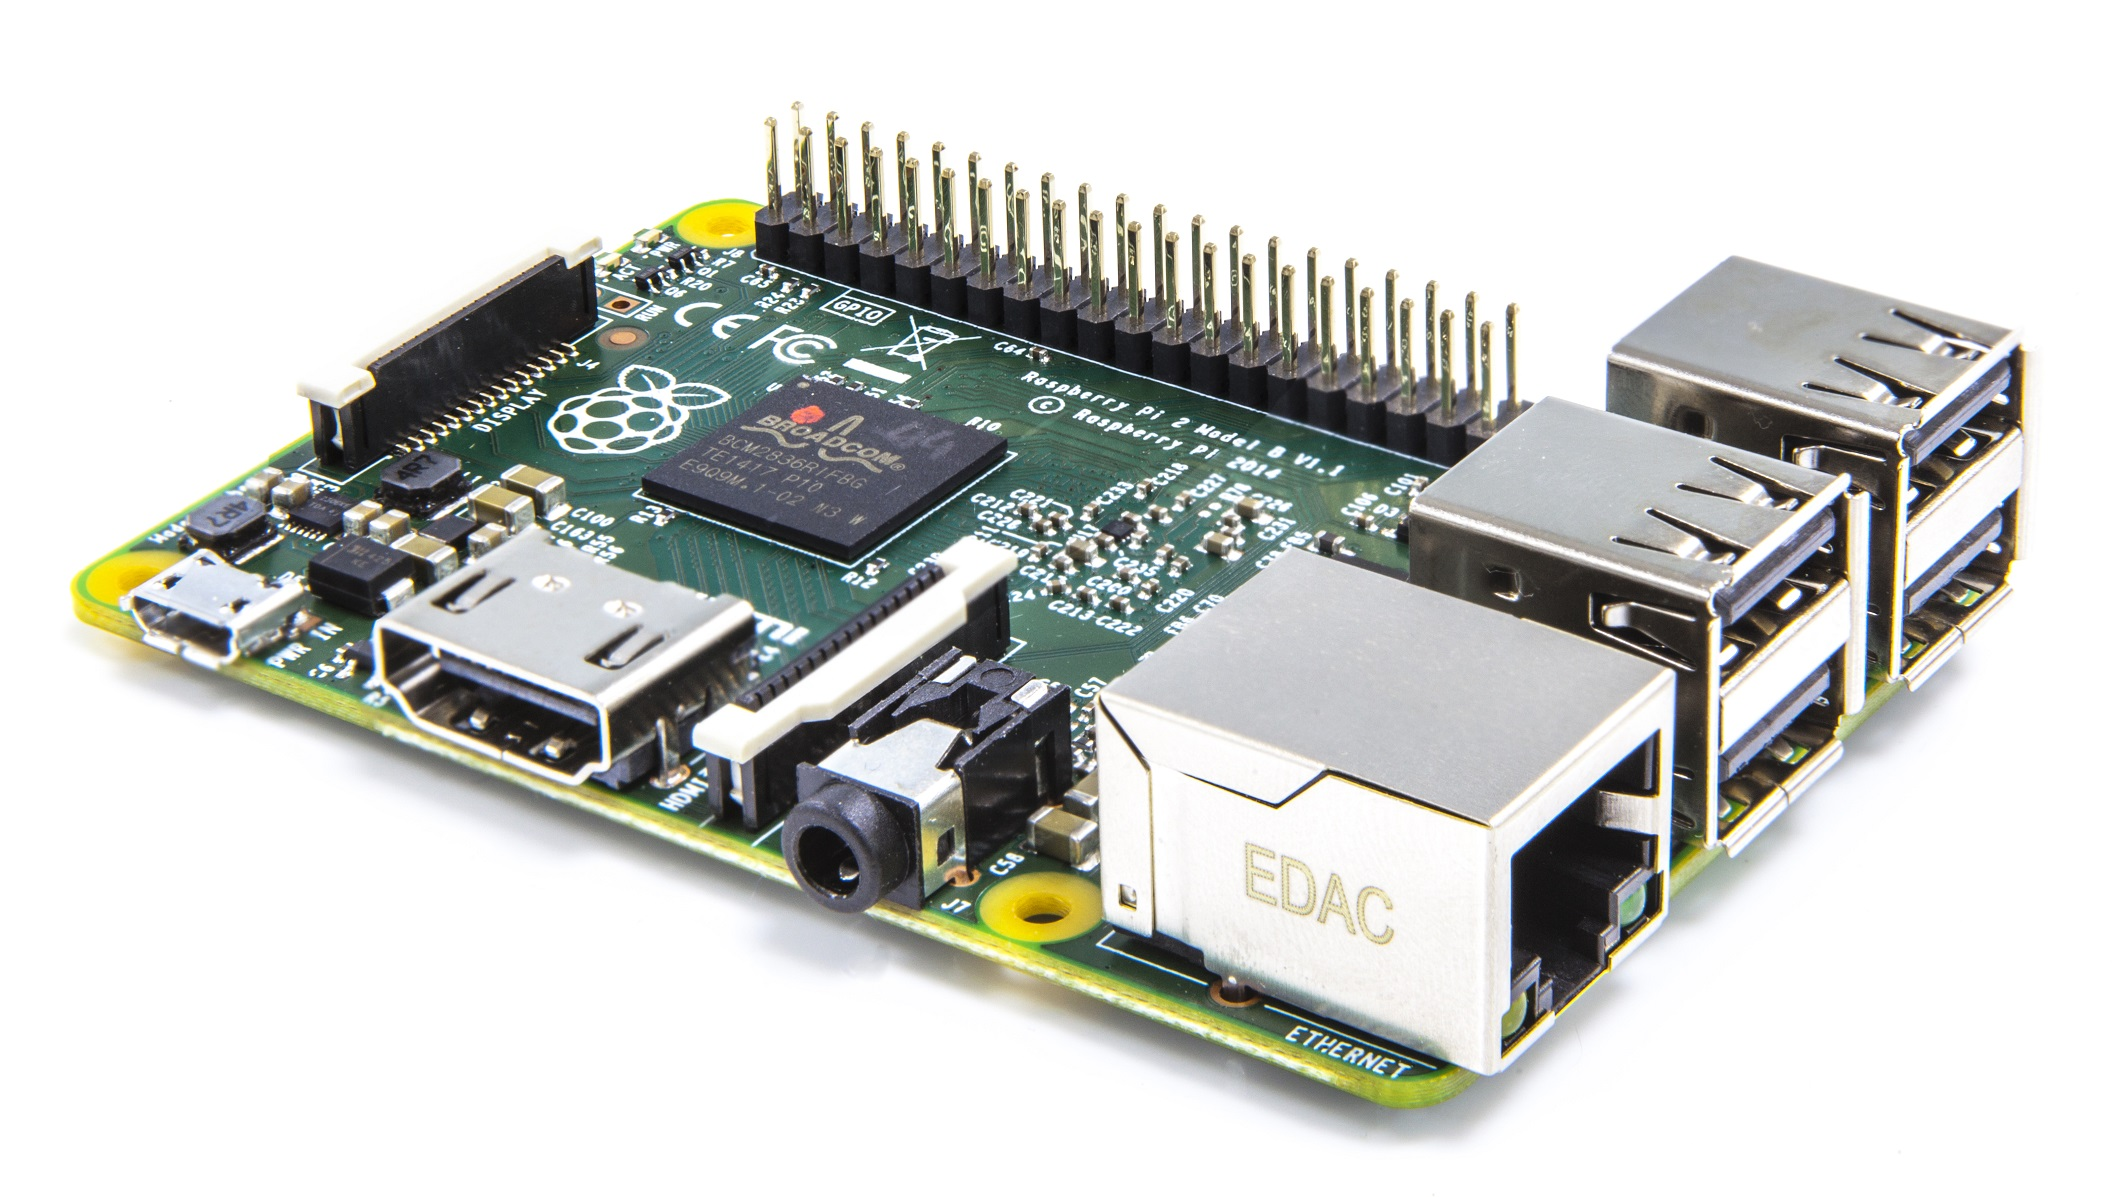
\includegraphics[width=0.7\linewidth]{img/raspberrypi2}
\end{minipage}\hfill
\begin{minipage}{0.32\linewidth}
 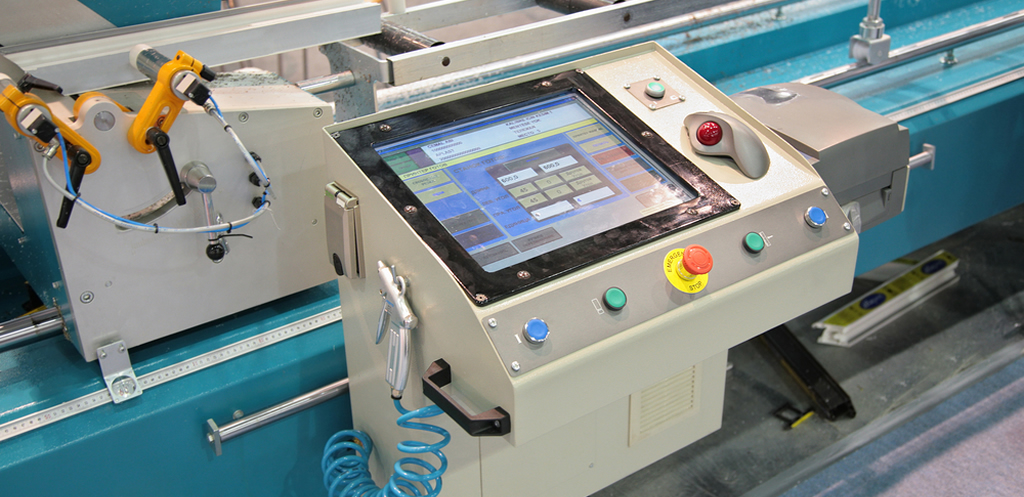
\includegraphics[width=0.7\linewidth]{img/infoindus}
\end{minipage}

~\

Ces systèmes correspondent à l'assemblage de plusieurs composants et possèdent sensiblement la même structure.
}}

{\frame{
\frametitle{Composants}

\begin{wrapfigure}[5]{l}{2cm}
\centering 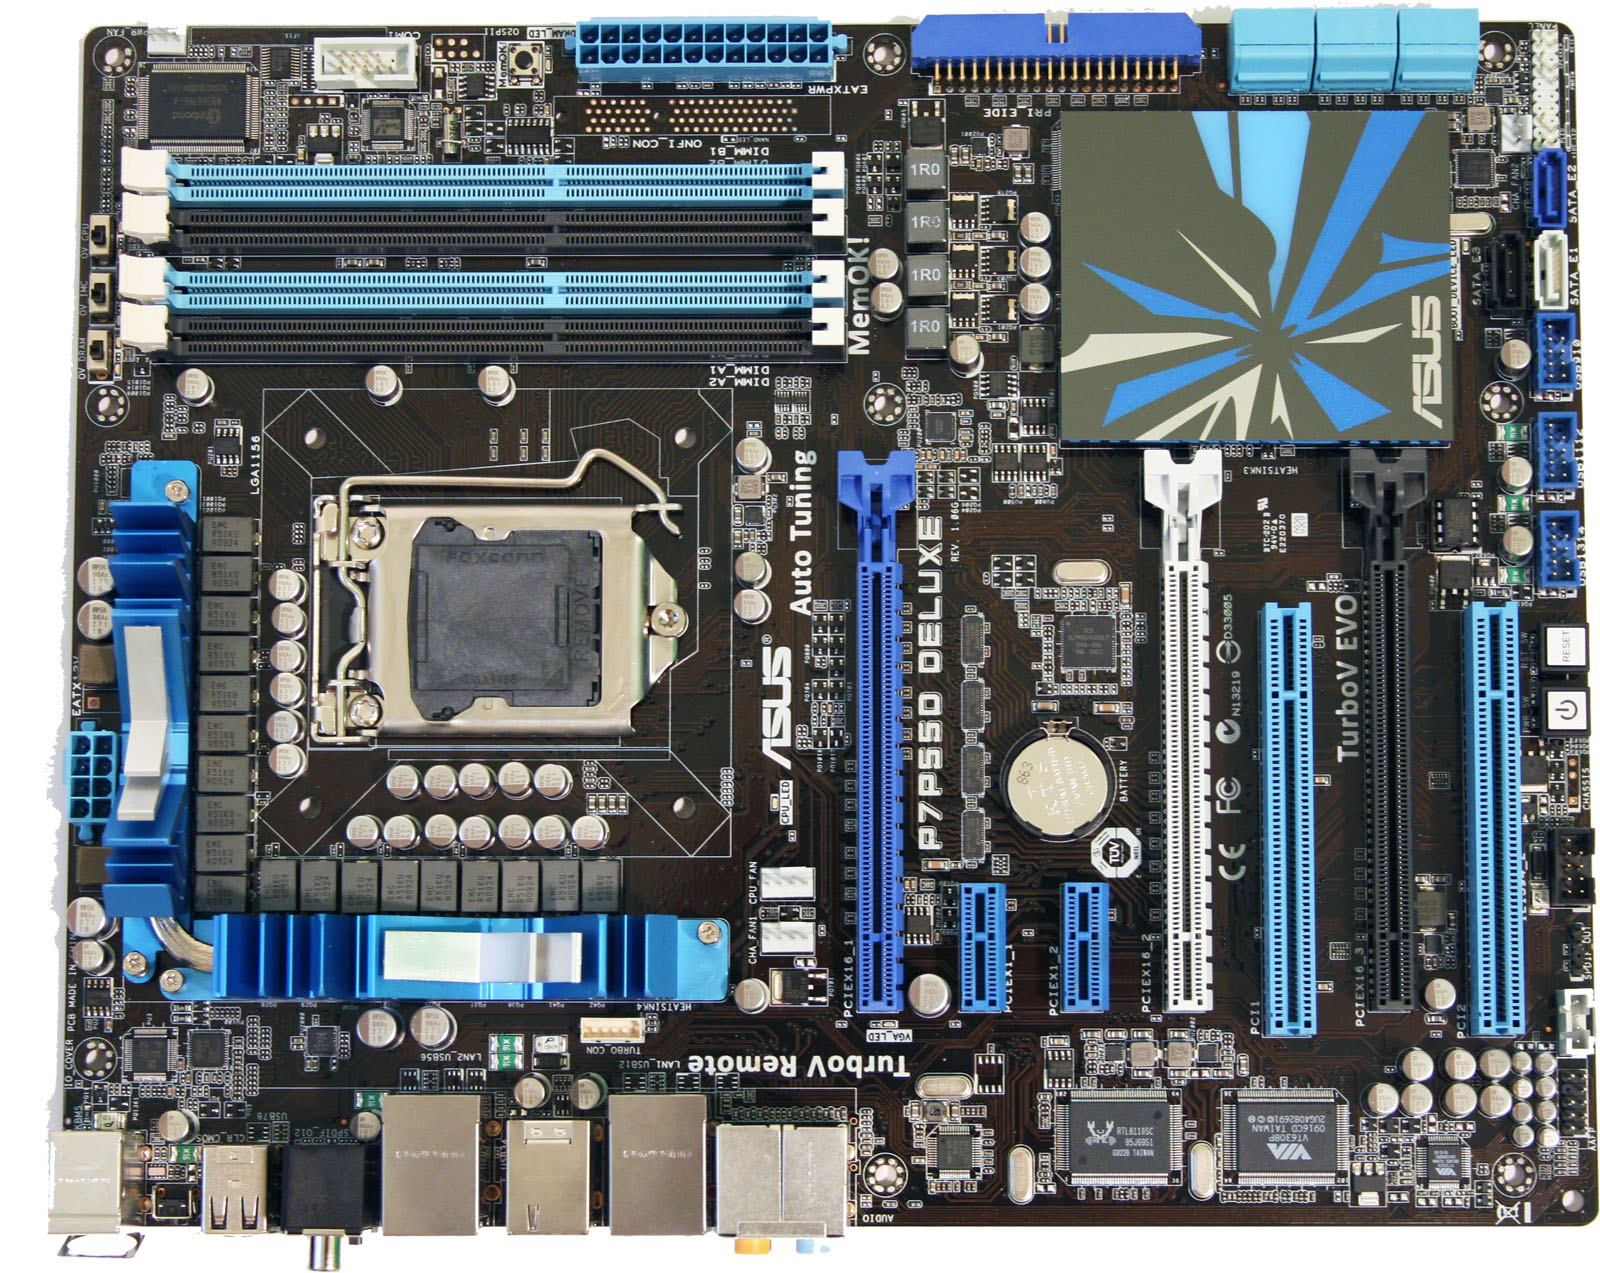
\includegraphics[width=\linewidth]{img/carte_mere}
\end{wrapfigure}

La \textbf{carte mère} est le c\oe ur de tout ordinateur.

Elle est essentiellement composée de circuits imprimés et de ports de connexion, par le biais desquels elle assure la connexion de tous les composants et périphériques propres à un micro-ordinateur (disques durs, mémoire vive, microprocesseur, cartes filles, etc.) afin qu'ils puissent être reconnus et configurés par la carte lors du démarrage.

\begin{wrapfigure}[4]{l}{2cm}
\centering 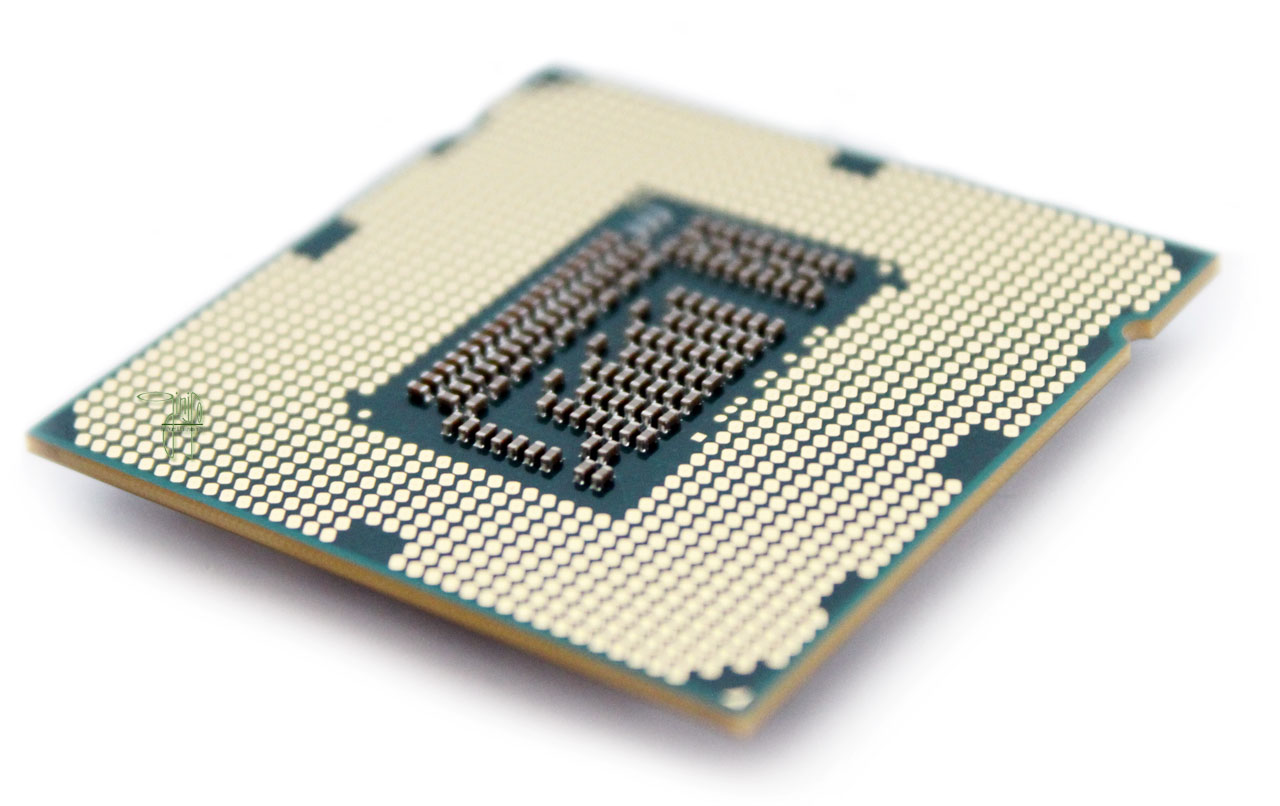
\includegraphics[width=\linewidth]{img/processeur}
\end{wrapfigure}

Le \textbf{processeur} a le rôle fondamental de la plupart des unités centrales de traitement, indépendamment de la forme physique qu'elles prennent, est d'exécuter une série d'instructions stockées appelées \og programme \fg.

Les instructions (parfois décomposées en micro instructions) et les données transmises au processeur sont exprimées en mots binaires (code machine). Elles sont généralement stockées dans la mémoire. Le séquenceur ordonne la lecture du contenu de la mémoire et la constitution des mots présentés à l'ALU (Arithmetic and Logical Unit) qui les interprète.
}}

{\frame{
\frametitle{Composants}

\begin{wrapfigure}[5]{l}{2cm}
\centering 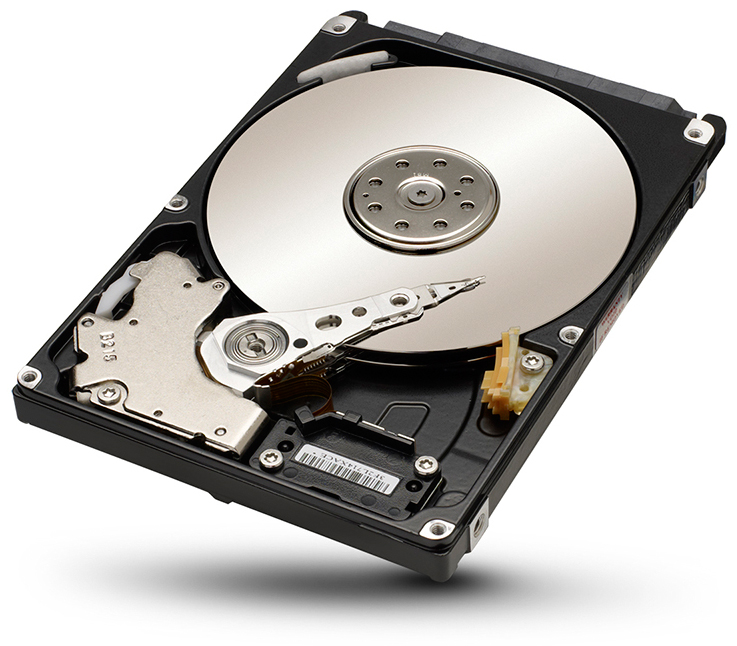
\includegraphics[width=\linewidth]{img/disque_dur}
\end{wrapfigure}

La \textbf{mémoire de masse} permet de stocker les données ainsi que les logiciels/applications installées.

Les données sont écrites en code binaire [0,1] sur le disque grâce à une tête de lecture/écriture. Suivant le courant électrique qui la traverse, cette tête modifie le champ magnétique local pour écrire soit un 1, soit un 0, à la surface du disque.

\begin{wrapfigure}[6]{l}{2cm}
\centering 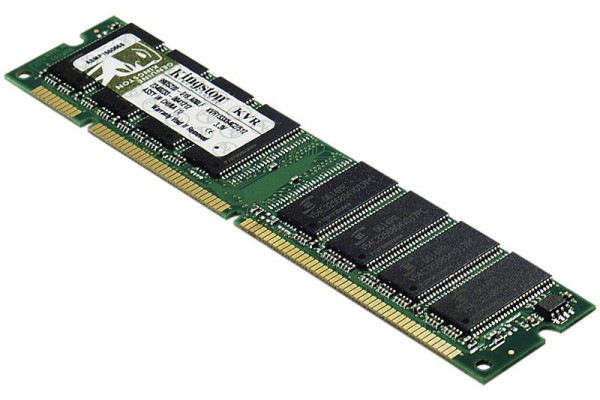
\includegraphics[width=\linewidth]{img/ram}
\end{wrapfigure}

La \textbf{mémoire vive}, ou mémoire système aussi appelée RAM de l'anglais Random Access Memory (que l'on traduit en français par mémoire à accès direct), est la mémoire informatique dans laquelle un ordinateur place les données lors de leur traitement.

}}

{\frame{
\frametitle{Composants}

\centering \includegraphics[width=\linewidth]{img/ordi}

}}

\section{Les systèmes d'exploitation} 

{\frame{
\frametitle{Système d'exploitation}

\begin{wrapfigure}[13]{r}{3cm}
\centering 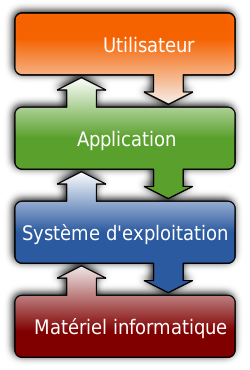
\includegraphics[width=\linewidth]{img/systeme_exploitation}
\end{wrapfigure}

En informatique, un système d'exploitation (souvent appelé OS pour Operating System, le terme anglophone) est un ensemble de programmes qui dirige l'utilisation des capacités d'un ordinateur par des logiciels applicatifs.

~\

Il reçoit de la part des logiciels applicatifs des demandes d'utilisation des capacités de l'ordinateur, capacité de stockage des mémoires et des disques durs, capacité de calcul du processeur, capacités de communication vers des périphériques.

~\

Le système d'exploitation accepte ou refuse de telles demandes, puis réserve les ressources en question pour éviter que leur utilisation n'interfère avec d'autres demandes.


}}

{\frame{
\frametitle{Rôles du système d'exploitation}

\begin{itemize}
 \item \textbf{Gestion du processeur:} le système d'exploitation est chargé de gérer l'allocation du processeur entre les différents programmes grâce à un algorithme d'ordonnancement.
 \item \textbf{Gestion de la mémoire vive:} le système d'exploitation est chargé de gérer l'espace mémoire alloué à chaque application et, le cas échéant, à chaque usager.
 \item \textbf{Gestion des entrées/sorties:} le système d'exploitation permet d'unifier et de contrôler l'accès des programmes aux ressources matérielles par l'intermédiaire des pilotes (écran, clavier, souris, imprimante,...),
 \item \textbf{Gestion de l'exécution des applications:} le système d'exploitation est chargé de la bonne exécution des applications en leur affectant les ressources nécessaires.
 \item \textbf{Gestion des droits:} le système d'exploitation garantit que les ressources ne sont utilisées que par les programmes et utilisateurs possédant les droits adéquats.
 \item \textbf{Gestion des fichiers:} le système d'exploitation gère la lecture et l'écriture dans le système de fichiers et les droits d'accès aux fichiers par les utilisateurs et les applications.
 \item \textbf{Gestion des informations:} le système d'exploitation fournit un certain nombre d'indicateurs permettant de diagnostiquer le bon fonctionnement de la machine.
\end{itemize}
}}

{\frame{
\frametitle{Composantes du système d'exploitation}

Le système d'exploitation est composé d'un ensemble de logiciels permettant de gérer les interactions avec le matériel. Parmi cet ensemble de logiciels on distingue généralement les éléments suivants :
\begin{itemize}
 \item Le \textbf{noyau} (en anglais kernel) représentant les fonctions fondamentales du système d'exploitation telles que la gestion de la mémoire, des processus, des fichiers, des entrées-sorties principales, et des fonctionnalités de communication.
 \item L'\textbf{interpréteur de commande} (en anglais shell, traduisez \og coquille \fg par opposition au noyau) permettant la communication avec le système d'exploitation par l'intermédiaire d'un langage de commandes, afin de permettre à l'utilisateur de piloter les périphériques en ignorant tout des caractéristiques du matériel qu'il utilise, de la gestion des adresses physiques, etc.
 \item Le \textbf{système de fichiers} (en anglais \og file system \fg, noté FS), permettant d'enregistrer les fichiers dans une arborescence.
\end{itemize}
}}

{\frame{
\frametitle{Les principaux systèmes d'exploitation}

\begin{center}
\begin{tabular}{|c|c|c|}
\hline
Système	& Codage & Logo \\
\hline
Windows & 32/64 bits & 
\includegraphics[height=1.5cm]{img/windows10} \\
\hline
GNU/Linux (UNIX) & 32/64 bits & 
\includegraphics[height=1.5cm]{img/linux} \\
\hline
MAC OS X (UNIX) & 32 bits & 
\includegraphics[height=1.5cm]{img/mac} \\
\hline
\end{tabular}
\end{center}

}}

\end{document}